

\section{5. Preliminary Project}

\subsection{5.1 Aims}
\begin{enumerate}
    \item Disease Detection and Tracking: The web application will allow users equipped with mobile devices and GPS capabilities to perform visual inspections of vineyards and detect three types of vine diseases (A, B, and C). Users can input the disease type, position, date, and time of detection.

    \item Geospatial Visualization: The application will utilize the UTM WGS84 reference system to accurately represent the geographical distribution of vineyard areas and individual vineyards. Geospatial data will be visualized on an interactive map, enabling users to easily locate specific areas and vineyards.

    \item Vineyard Management: Users will be able to manage their vineyard data, including area codes, vineyard numbering, year of planting, and vine types. This information will be stored in a structured manner to facilitate effective disease tracking and intervention planning.

    \item Treatment Planning and Monitoring: Based on disease detection and other variables, the application will provide recommendations for necessary interventions or treatments. Users can log the treatments applied, which will be associated with specific vineyards. The application will also support remote monitoring of treatment effectiveness using aerial imagery captured by the hexacopter's azimuthal camera.

    \item Data Integration: The application will enable users to upload shape files containing geometries and attributes of their vineyard areas and vineyards. The system will process and store this data, ensuring it is accessible for disease monitoring and analysis.

    \item User Collaboration: As the application serves multiple customer companies, it will support user accounts with varying levels of access and permissions. Agronomists and farm personnel from different companies can collaborate by sharing disease detection information and treatment outcomes.

    \item Reporting and Insights: The application will generate reports summarizing disease occurrences, treatment histories, and intervention effectiveness. These reports will help agronomists and farm managers make informed decisions to optimize vineyard health.

    \item Automated Alerts: The application will have the capability to send automated alerts to users when disease detections are recorded, ensuring timely responses and interventions.

    \item Scalability and Global Compatibility: The application will be designed to accommodate the firm's widespread customer base, ensuring compatibility with different countries, languages, and regulations.

    \item User-Friendly Interface: The web application will feature an intuitive and user-friendly interface, making it accessible to agronomists and farm personnel with varying levels of technical expertise.
\end{enumerate}

\subsection{5.2 Functions of the System}
\begin{enumerate}

    \item \textbf{Display mode}
          \begin{itemize}
              \item Dark mode/Bright mode: By toggling the button on the right side of the navigation bar, the pages will be displayed in two modes.

                    \begin{figure}
                        \centering
                        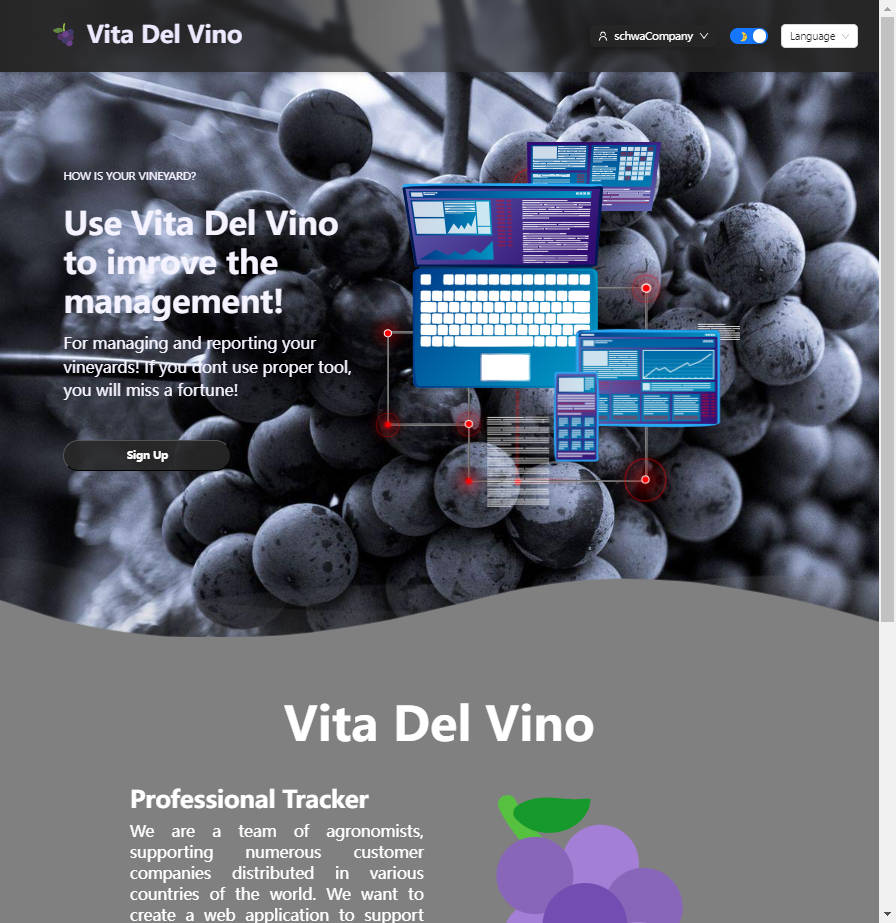
\includegraphics[width=1\linewidth]{images/LandingPageDarkMode.jpg}
                        \caption{Landing Page in Dark Mode}
                        \label{fig:LandingPageDarkMode}
                    \end{figure}
              \item Languages: This website can be displayed in three languages by toggling the language options, namely, Italian, Chinese, and English.
          \end{itemize}
    \item \textbf{User functions}
          \begin{itemize}
              \item User log-in
                    Users for this website including company users (we call them users in this report)  and an agronomist can log into the website by username and password. From this page, the user can also go to the register page by clicking the text.
                    \begin{figure}
                        \centering
                        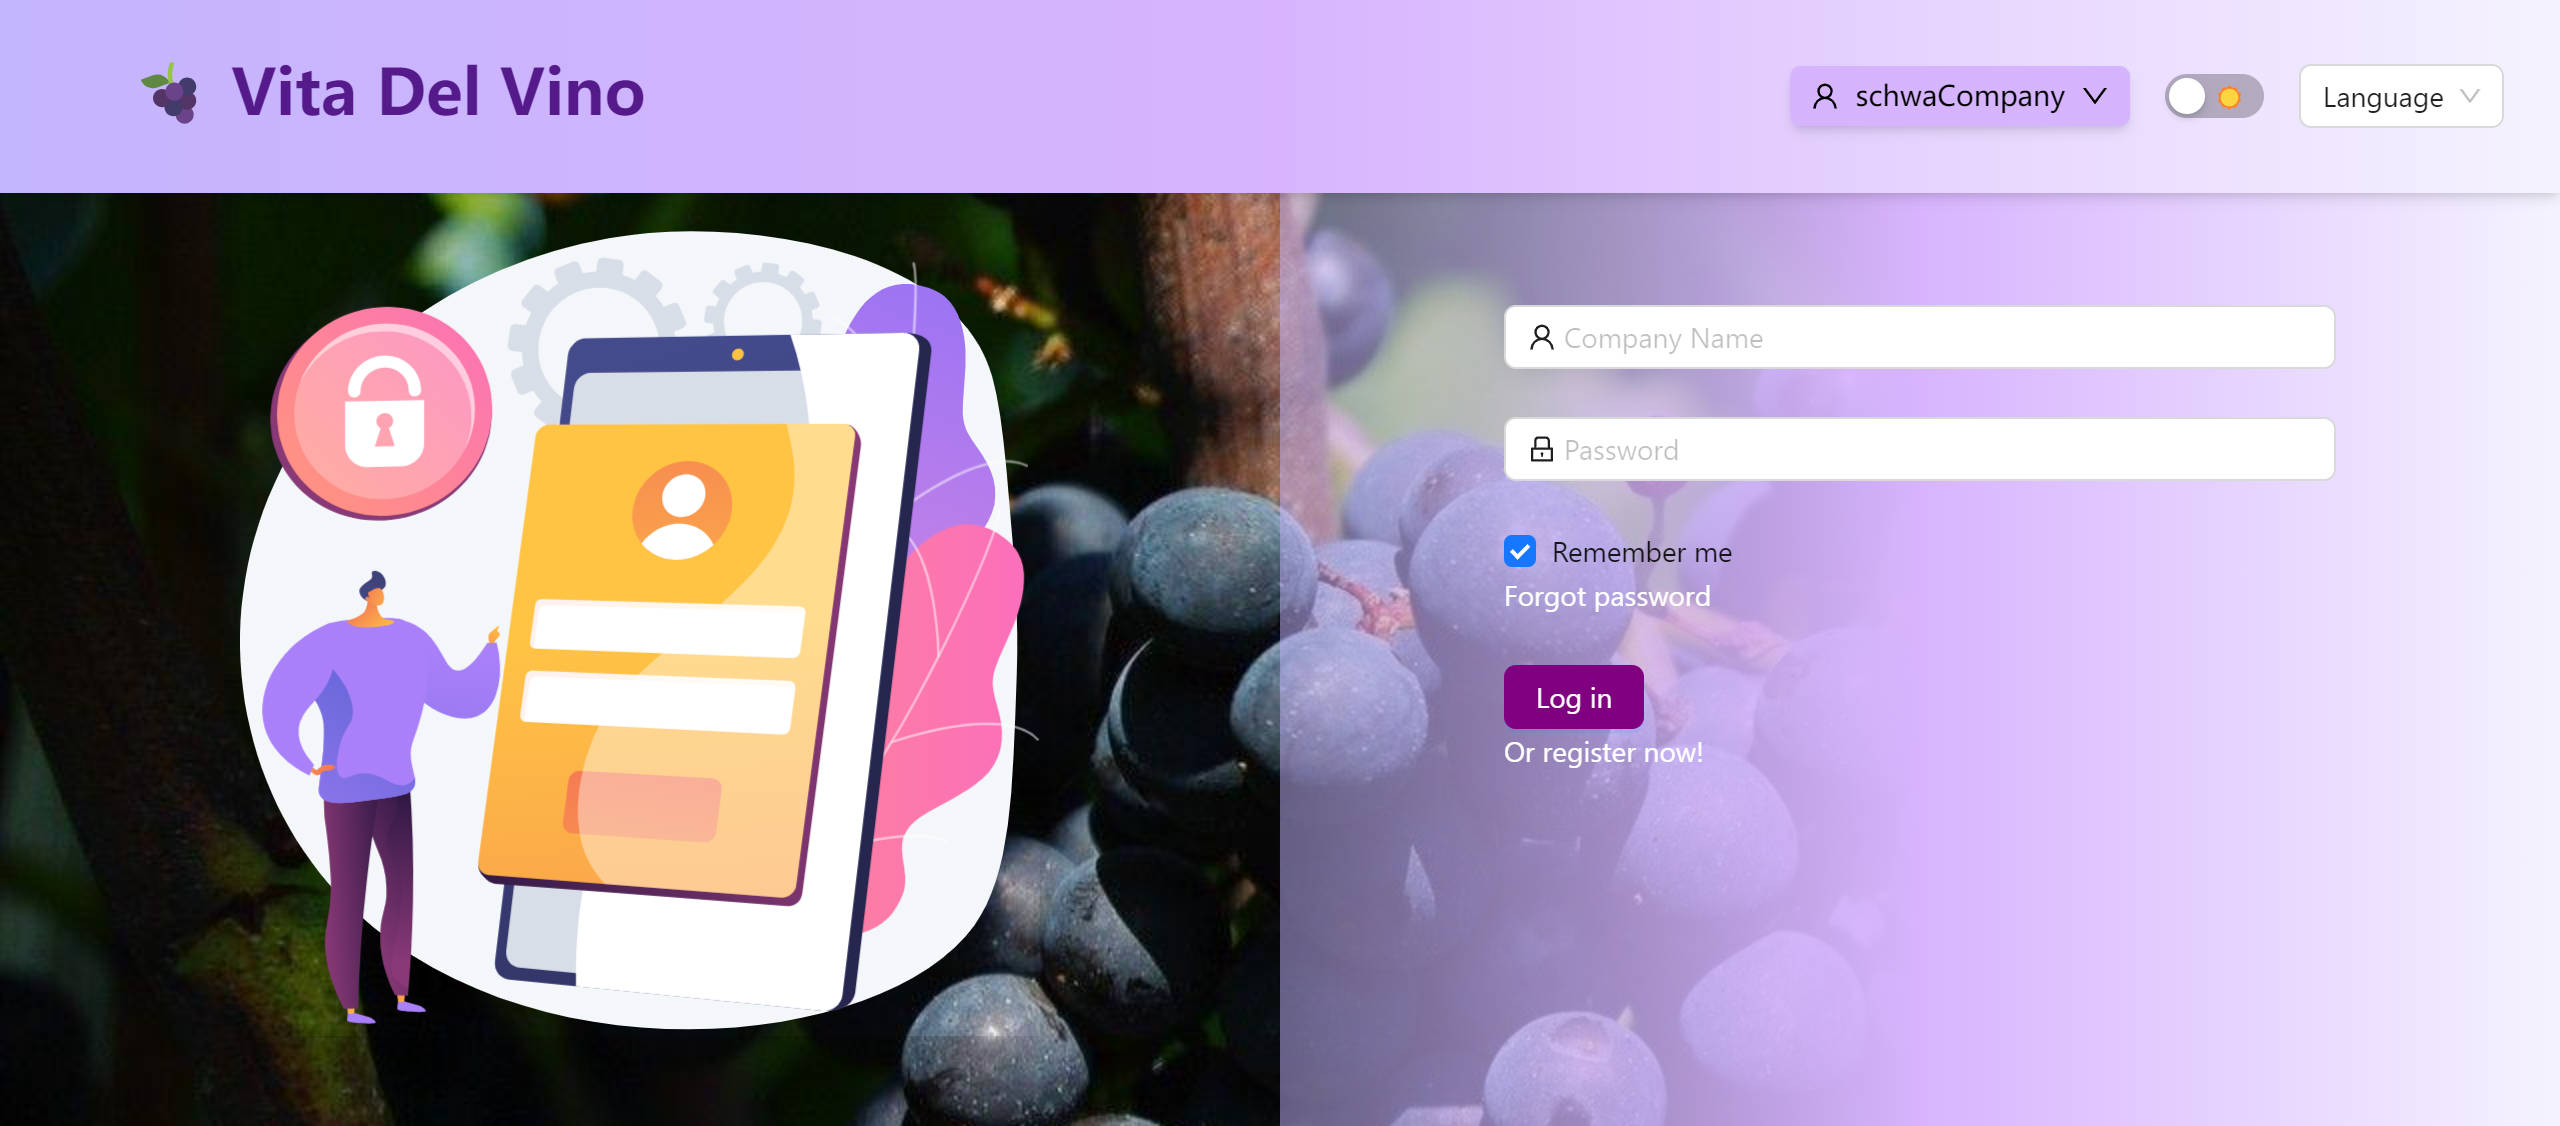
\includegraphics[width=0.75\linewidth]{images/Login.jpg}
                        \caption{User Log in}
                        \label{fig:Login}
                    \end{figure}
              \item User log out
                    Users typically initiate the logout process by clicking on a "Logout" button on the dropdown navigation menu. Upon clicking the "Logout" button, the user's current session is terminated. This means that they are no longer authenticated, and their access to protected areas or features is revoked.
                    \begin{figure}
                        \centering
                        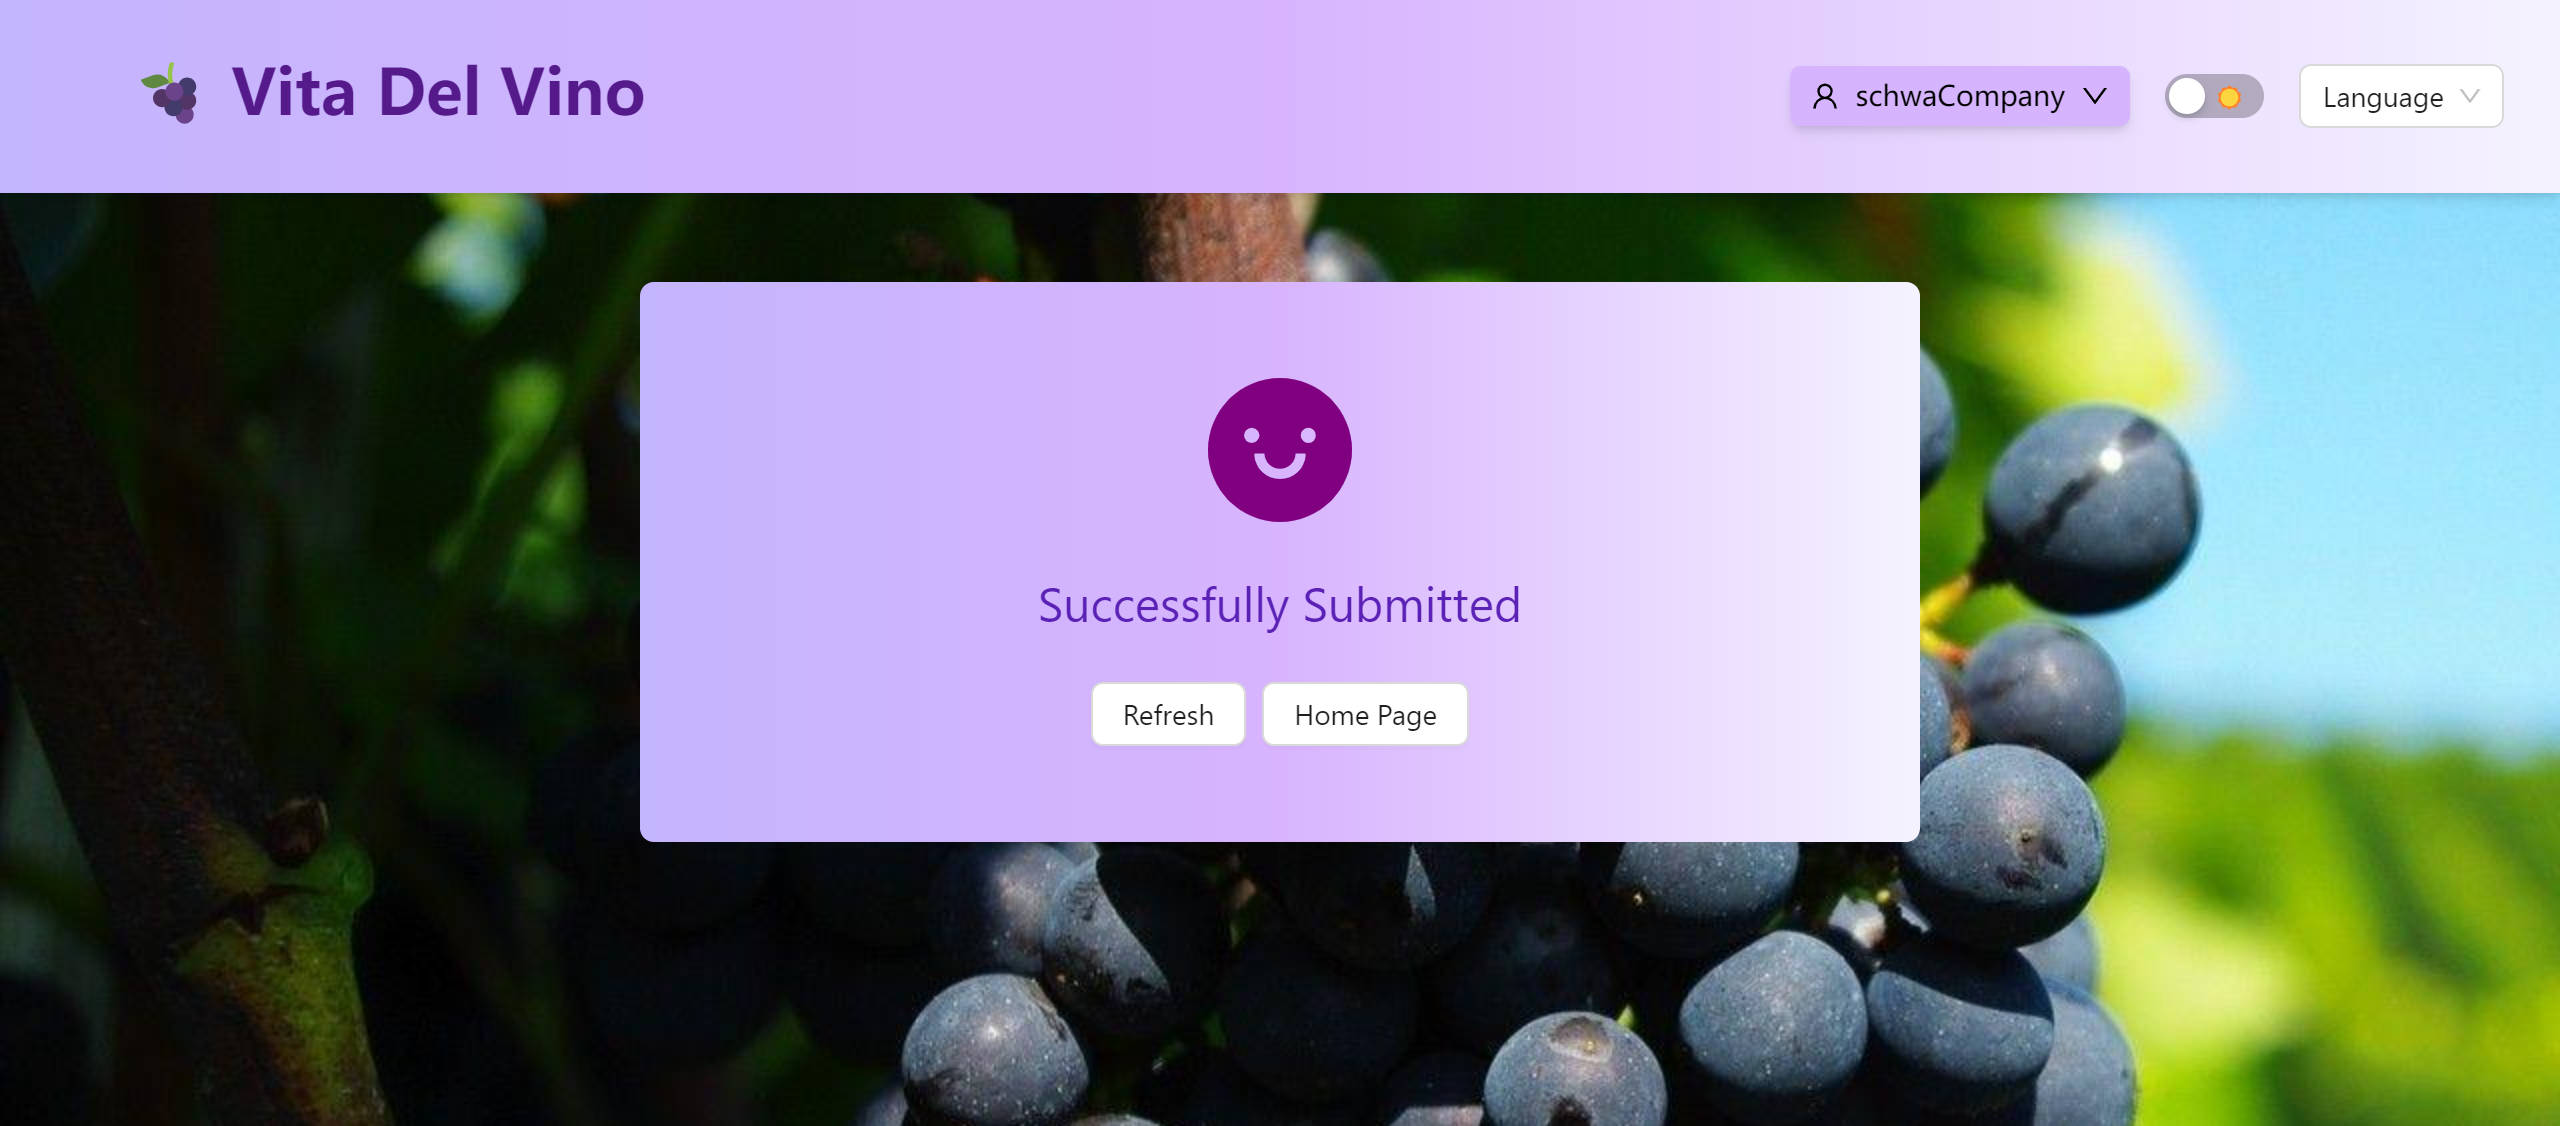
\includegraphics[width=0.75\linewidth]{images/Logout.jpg}
                        \caption{Logout}
                        \label{fig:Logout}
                    \end{figure}
              \item User sign up
                    Users can sign up by adding information.User sign-up is the process by which new users create accounts on the website.  Users access the registration form by clicking on a "Sign Up" on the drop down menu or "Register" link in the main page. The registration form collects essential information from the user.
                    \begin{figure}
                        \centering
                        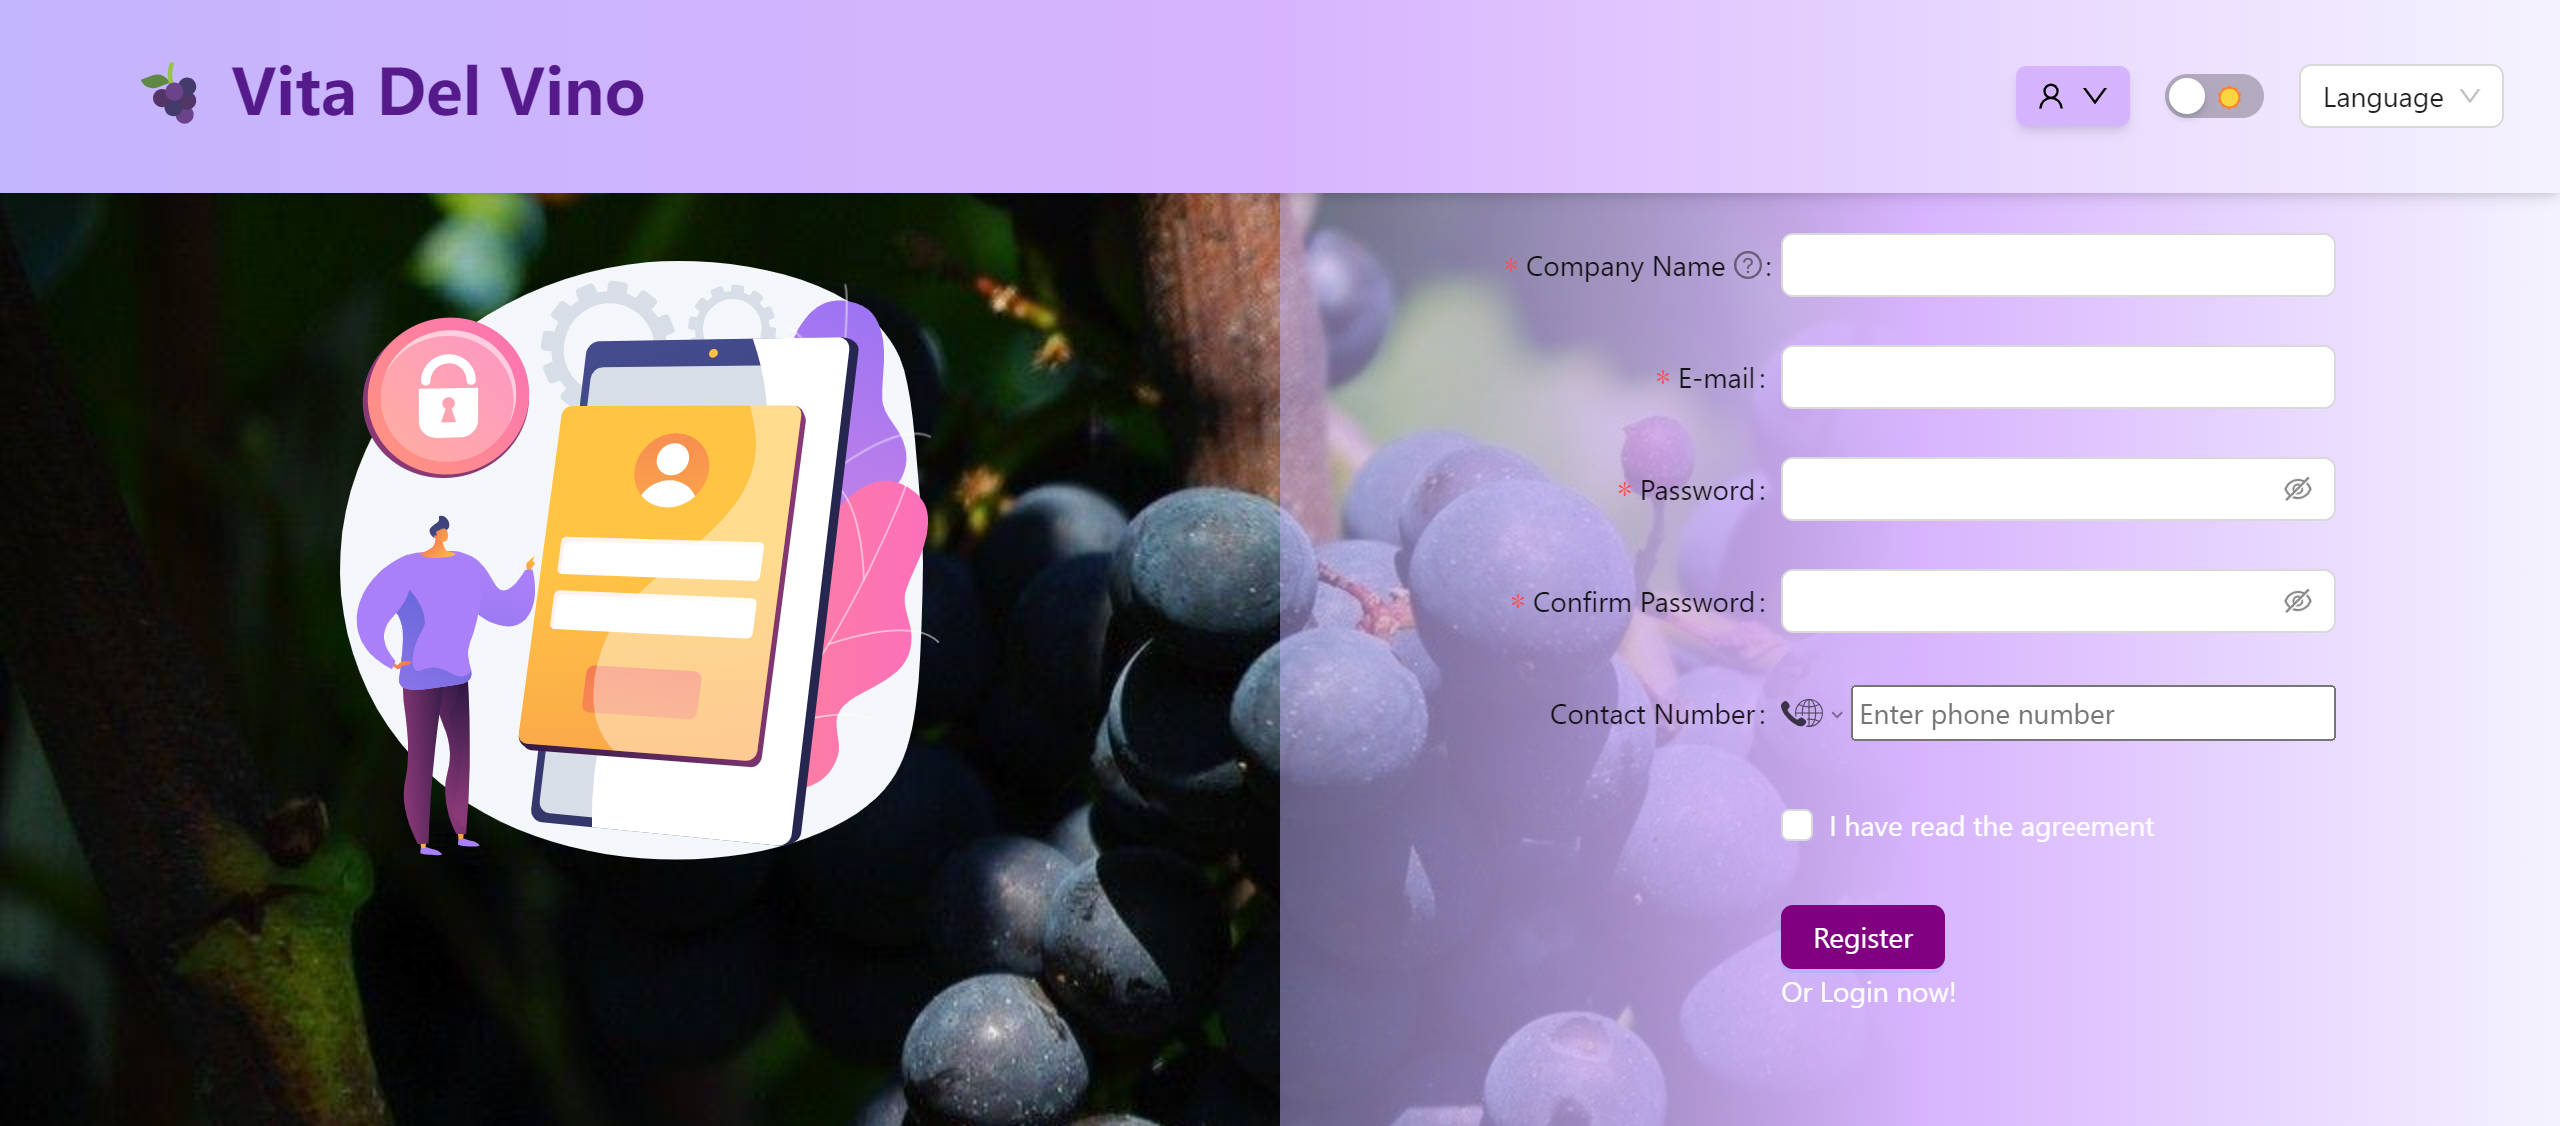
\includegraphics[width=0.75\linewidth]{images/SignUp.jpg}
                        \caption{Sign Up Page}
                        \label{fig:SignUp}
                    \end{figure}

                    As mentioned previously, users may need to specify their user type during sign-up by user name, distinguishing between company users and agronomists. Users are required to provide information such as their name, email address, contact details, and any other relevant information as per the website's requirements. Users choose a unique username and create a secure password for their account during sign-up. Password strength requirements and validation should be enforced. Users may be required to accept the website's terms and conditions, privacy policy, or user agreements as part of the sign-up process. After successfully completing the registration form and email verification (if applicable), users receive a confirmation message indicating that their account has been created. This message may include login instructions.

              \item   User settings
                    \begin{enumerate}
                        \item Edit user information: The user can change the information including the Company name and phone number.
                    \end{enumerate}
                    \begin{figure}
                        \centering
                        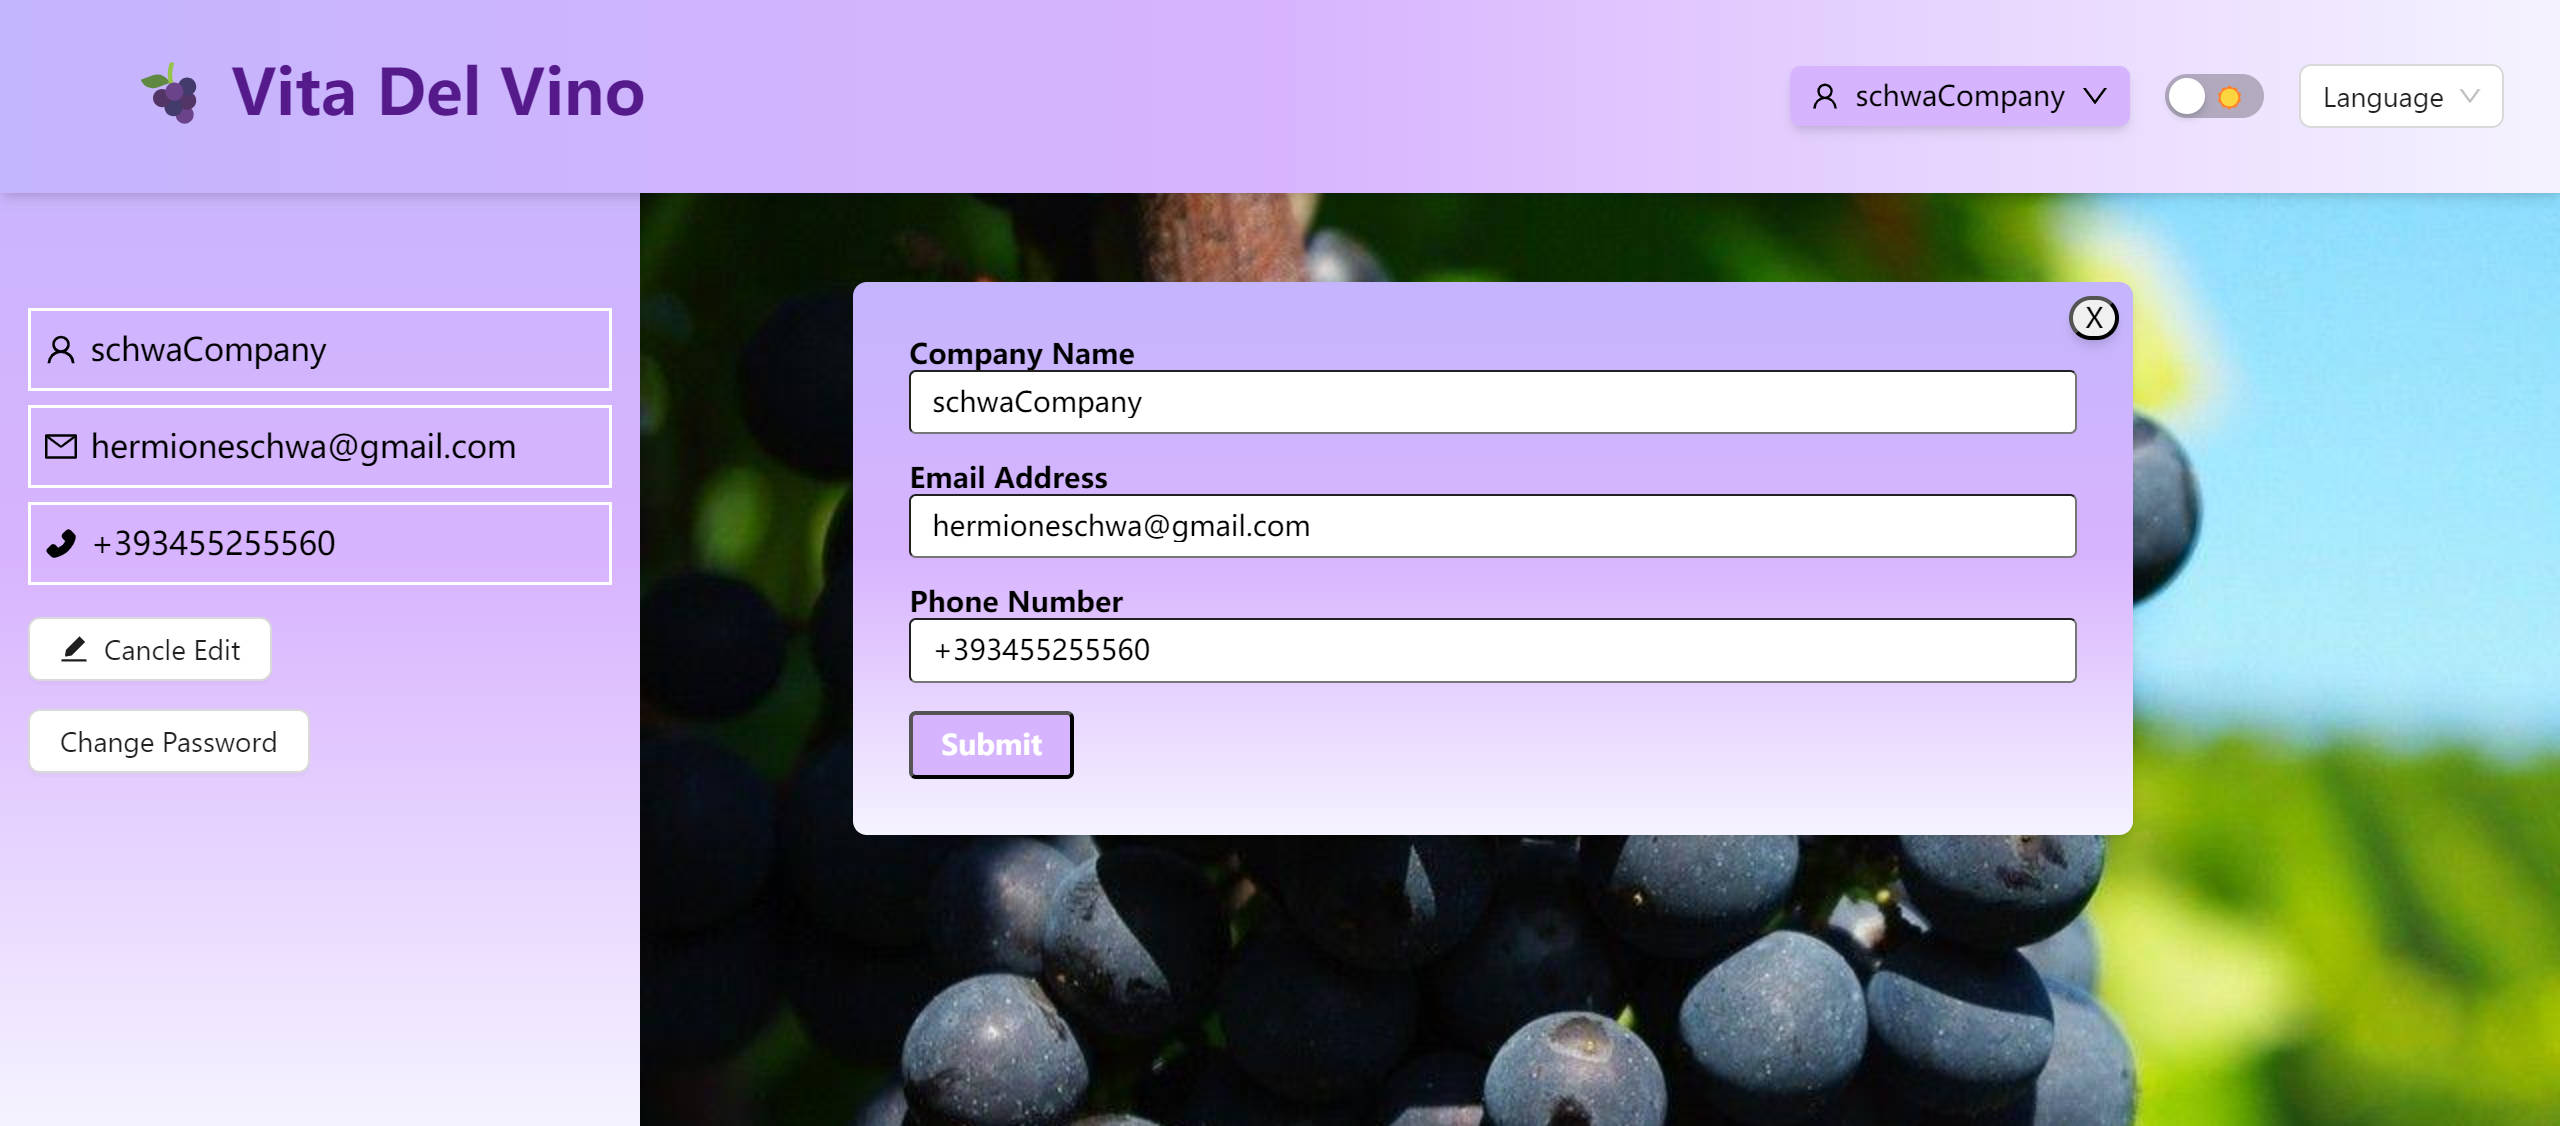
\includegraphics[width=0.75\linewidth]{images/UserSetting.jpg}
                        \caption{UserSetting Page}
                        \label{fig:UserSetting}
                    \end{figure}
                    \begin{enumerate}
                        \item Change the password: changing the password requires the user to verify the old password first. Once the password is confirmed by the website, the user can continue change the password to a new one.
                    \end{enumerate}
          \end{itemize}
    \item \textbf{Add new items}
          \begin{itemize}
              \item Add new reports

                    To add new reports, start by clicking the operation dropdown and selecting "Add a New Report." Once done, click the "Add Report" button to access the main page containing the report form. Within the form, begin by selecting the relevant area and specifying the associated vineyard.

                    \begin{figure}
                        \centering
                        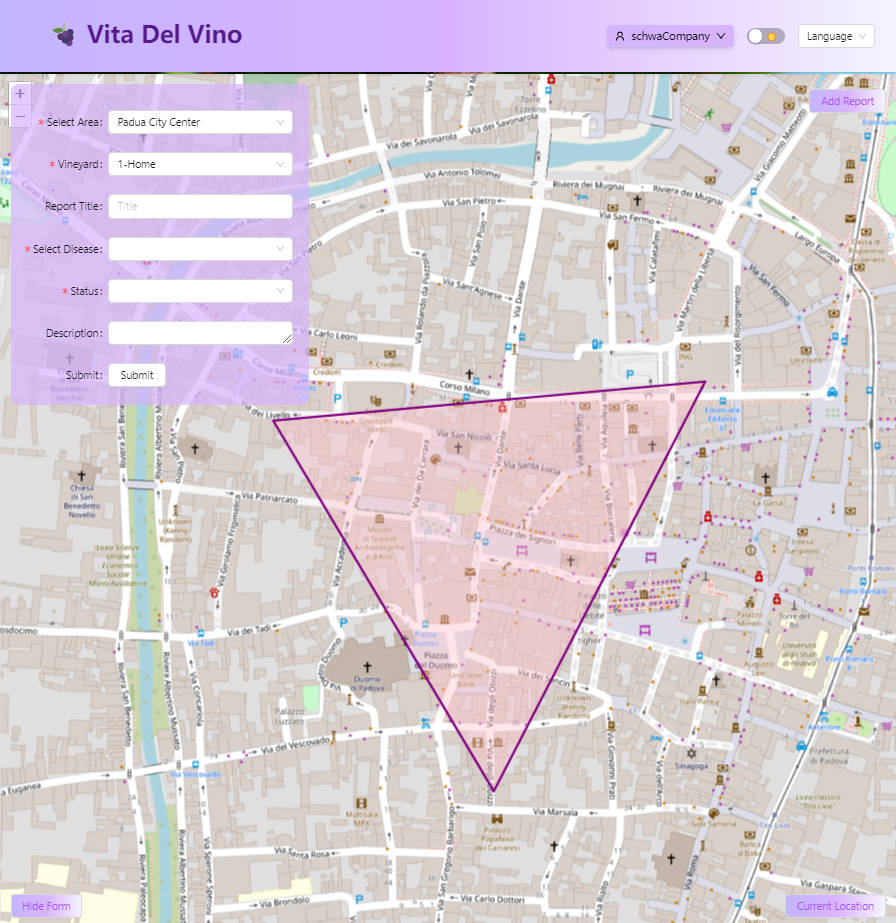
\includegraphics[width=1\linewidth]{images/AddReport.jpg}
                        \caption{Add Report}
                        \label{fig:AddReport}
                    \end{figure}

                    To provide report details, click the "Edit a Report" button, where you can input the report title, choose a disease from the dropdown menu, and set the status (defaulted to 'New Report'). Add a comprehensive description to the report, then finalize by clicking "Submit" to send all data to the database. A successful submission prompts an information box confirming the action, offering options to return to the main page or refresh the current one. This streamlined process ensures efficient addition of new reports while facilitating seamless data contribution.


              \item Add new items
                    \begin{enumerate}
                        \item Add new area

                              Adding a new area within the system is a valuable function for users who want to categorize and organize their agricultural data geographically. Here's how this feature works:
                              \begin{itemize}
                                  \item Area Definition: Users can define a new agricultural area within the system. This could represent a specific piece of land, a farm, or any other geographical designation relevant to their agricultural operations.

                                  \item Geospatial Data: Users may have the option to specify the location of the new area using geospatial data such as coordinates, addresses, or interactive maps. This feature can be particularly useful for precision agriculture, where accurate location data is crucial.

                                  \item Area Details: Users can provide additional details about the new area, including its size, soil type, climate conditions, and any other relevant information. These details help in comprehensive agricultural management and planning.

                                  \item Customization: The system may allow users to customize the naming and categorization of the new area, making it easier to identify and manage within the application.

                                  \item Associated Data: Users can associate other data with the newly added area, such as crop types, planting dates, and yield records. This helps in tracking and analyzing agricultural activities specific to that area.
                              \end{itemize}
                        \item Add new vineyard
                              \begin{figure}[htbp]
                                  \centering
                                  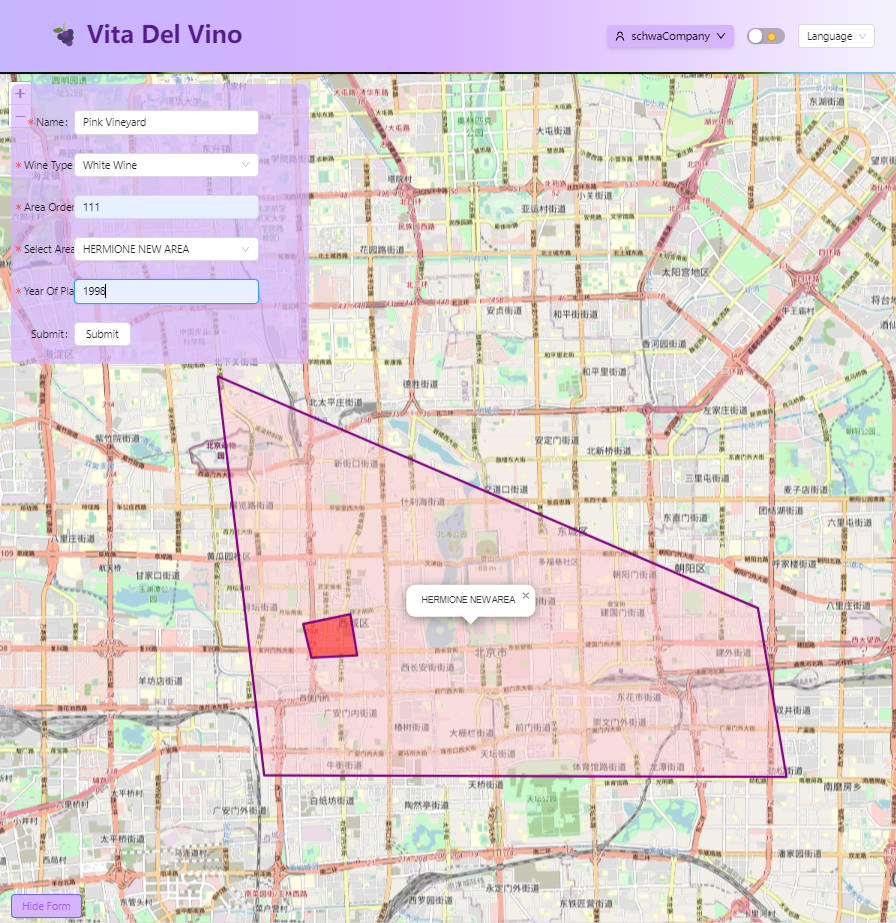
\includegraphics[width=\textwidth]{images/AddNewVineyard.jpg}
                                  \caption{AddNewVineyard}
                                  \label{fig:AddNewVineyard}
                              \end{figure}

                              For users involved in viticulture or grape cultivation, the ability to add new vineyards is a critical aspect of the system. Here's how this feature enhances vineyard management:

                              \begin{itemize}
                                  \item Vineyard Creation: Users can create a new vineyard profile, specifying details such as the vineyard's name, location, and size. This information is crucial for monitoring and optimizing grape production.

                                  \item Grape Varieties: Users can associate specific grape varieties with the vineyard, allowing for precise tracking of grape types and their characteristics.

                                  \item Vineyard Layout: Some systems may offer tools for designing and visualizing the layout of the vineyard, including row configurations, trellis systems, and irrigation setups.

                                  \item Pest and Disease Monitoring: Integrated pest and disease monitoring features can help users track and manage threats to the vineyard's health, enabling timely interventions to protect the grape crop.
                              \end{itemize}
                    \end{enumerate}
          \end{itemize}
      \item  edit items      
          \begin{enumerate}
              \item Edit reports
                    \begin{enumerate}

                        \item  As a User:

                              As a user of the system, you have the ability to interact with reports in several ways to ensure accurate and up-to-date information:
                              \begin{itemize}

                                  \item Edit Report Information:

                                        Users have the capability to edit the information contained in a report. This flexibility is crucial for maintaining the accuracy and relevance of the data within the system. When circumstances change or additional details need to be included, users can update the report's content.

                                  \item Change Report Status and Leave Actions:

                                        After receiving feedback from agronomists or assessing the situation, users can modify the status of a report. This change in status reflects the current condition of the issue reported in the vineyard. Along with updating the status, users have the option to leave detailed information about the actions taken or planned. This transparency and communication ensure that all stakeholders are informed about the progress and resolutions related to the reported problem.

                                  \item Delete a Report (with Confirmation):

                                        Users also have the capability to delete a report if it's no longer relevant or necessary. However, this action should be carried out with caution, and the system typically prompts users to confirm their decision before permanently removing the report. This confirmation step prevents accidental data loss and encourages responsible data management.

                              \end{itemize}
                        \item  As an Agronomist:

                              Agronomists play a crucial role in providing guidance and expertise to address issues reported in vineyards. Here's how agronomists can interact with the system:
                              \begin{itemize}


                                  \item View and Evaluate Reports:

                                        Agronomists have access to reports submitted by users. They can thoroughly evaluate the information provided in the report, including details about disease outbreaks or other vineyard-related issues.

                                  \item Add Recommended Measures:

                                        After reviewing a report, agronomists can contribute their expertise by suggesting measures that could be taken to address the reported disease or problem. These measures may include recommended treatments, preventive actions, or specific interventions to mitigate the issue. Providing actionable advice helps users make informed decisions to improve vineyard health and productivity.

                              \end{itemize}


                    \end{enumerate}
          
  
         
              \item Edit area

                    Users can edit existing agricultural areas to ensure that the information remains accurate and up-to-date. Users can edit the Geospatial Data by editing the data from the input box. Thus, the page will update the information of the area according to the changing data. This functionality allows for customization and adaptation as agricultural landscapes change over time.

                    \begin{figure}
                        \centering
                        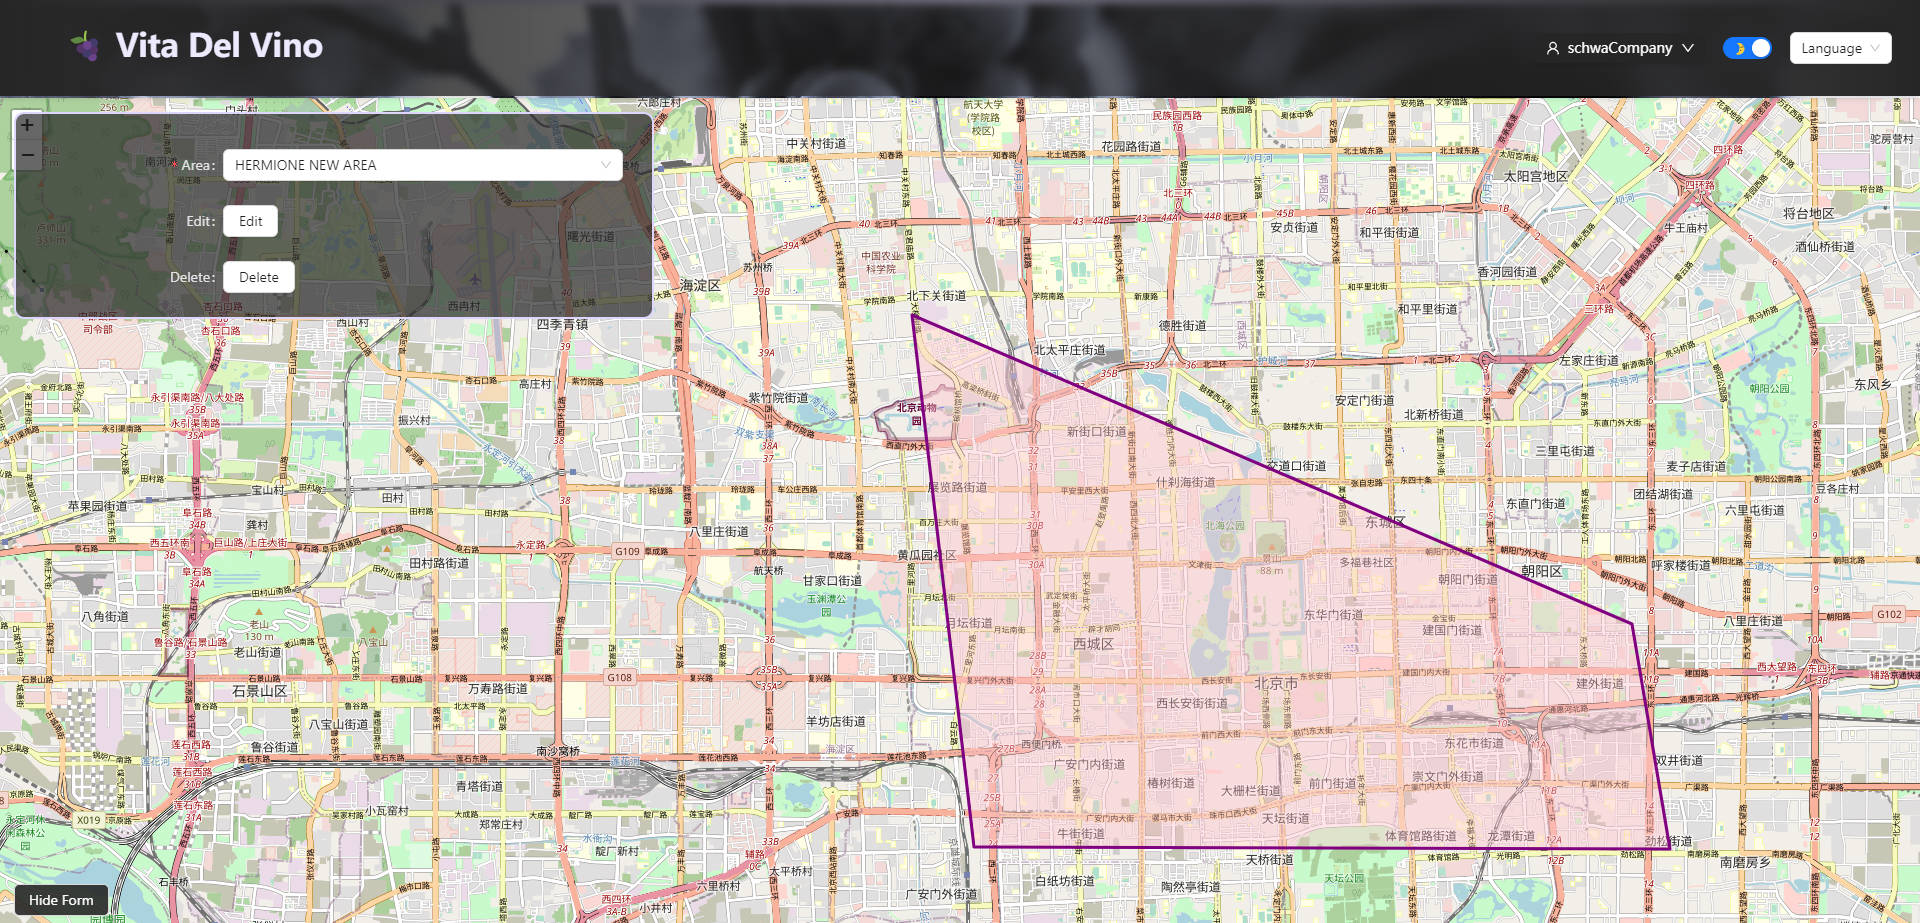
\includegraphics[width=1\linewidth]{images/EditArea.jpg}
                        \caption{Edit Area}
                        \label{fig:EditArea}
                    \end{figure}

              \item Edit vineyard
                    Users have the ability to edit vineyard information, which is crucial for managing vineyards effectively. This feature enables users to update details such as vineyard size, grape varieties planted, and any changes in vineyard layout or management practices.
       \end{enumerate}
    \item  List items
          \begin{enumerate}
              \item List reports
                    \begin{enumerate}
                        \item As a user:

                              Users can list reports that belong to them, providing a convenient way to review and track the issues they've reported. Additionally, users have the ability to filter reports by vineyard name, making it easier to organize and address specific concerns. The pagination function ensures that users can efficiently navigate through their reports, displaying a manageable number (e.g., five) of reports per page.

                                \begin{figure}
                                    \centering
                                    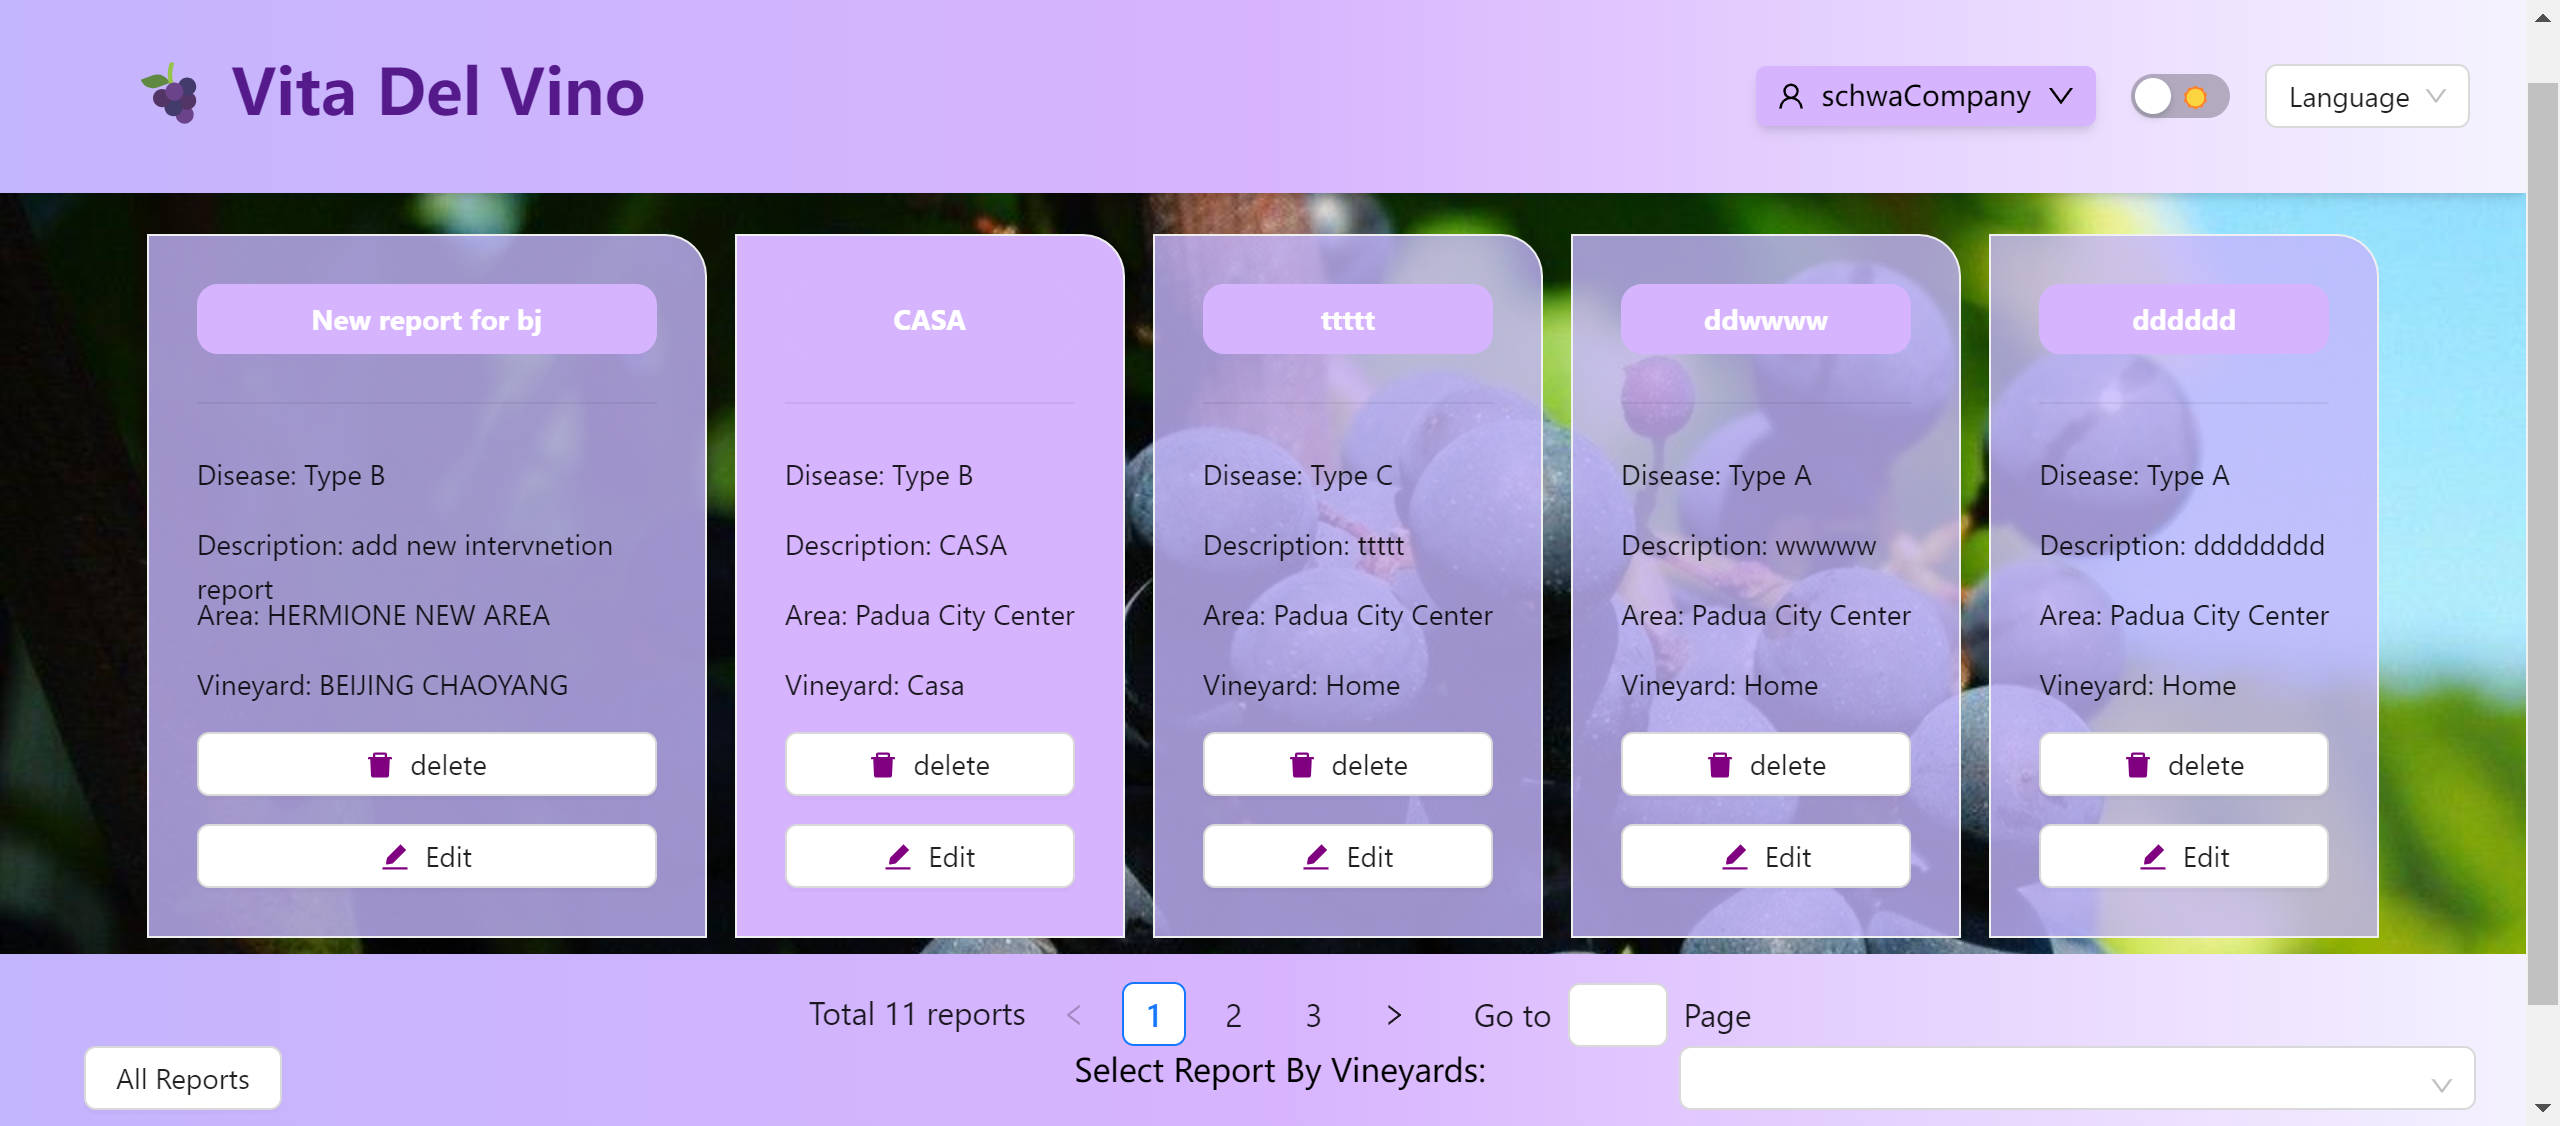
\includegraphics[width=1\linewidth]{images/ListReport.jpg}
                                    \caption{List Report}
                                    \label{fig:ListReport}
                                \end{figure}

                              
                        \item As an agronomist:

                              Agronomists, in their role as agricultural experts, can access and view all reports submitted by users. These reports contain valuable information about disease outbreaks, pest infestations, or other vineyard-related issues. Agronomists can use this information to assess the overall health of vineyards and provide targeted recommendations for intervention and improvement.

                              \begin{figure}
                                    \centering
                                    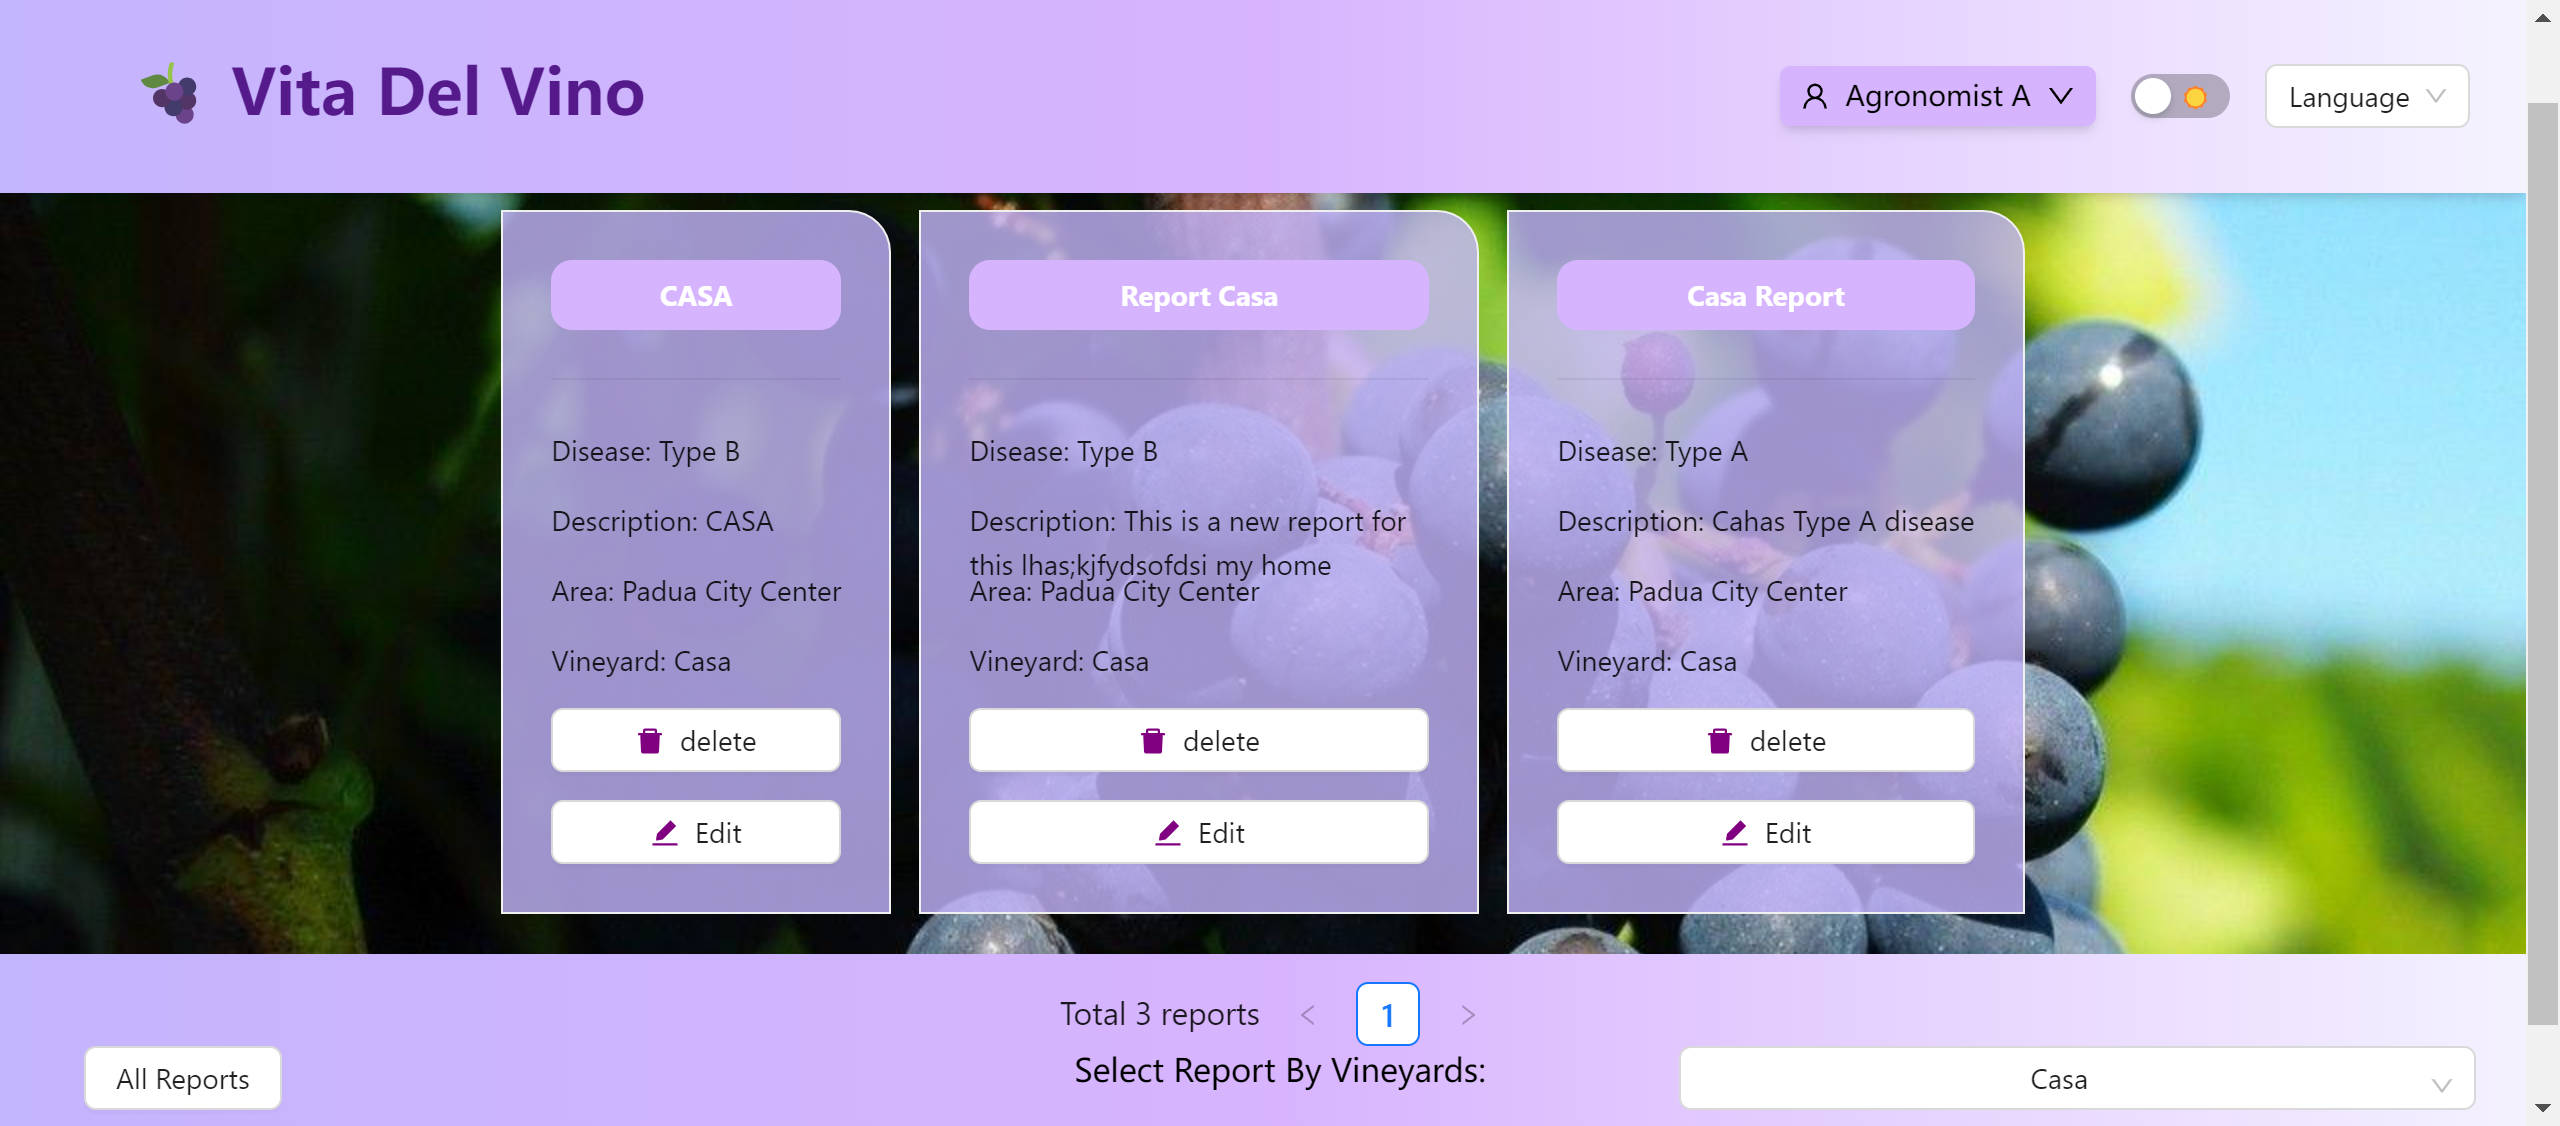
\includegraphics[width=1\linewidth]{images/ListReportAsAgo.jpg}
                                    \caption{List Report As Agronomist}
                                    \label{fig:ListReportAsAgo}
                                \end{figure}

                    \end{enumerate}
              \item List area
                    \begin{enumerate}
                        \item As a user

                              Users can list and access their designated agricultural areas. This feature is essential for keeping track of land parcels, farms, or agricultural zones under their management.


                        \item As an agronomist

                              Agronomists may use the list area function to view and evaluate agricultural areas associated with specific users or companies. This insight enables agronomists to provide informed recommendations for area-specific agricultural practices and improvements.

                    \end{enumerate}
              \item List vineyard
                    \begin{enumerate}
                        \item As a user
                              Users can list and access their registered vineyards, facilitating the management of grape-growing operations. This feature includes details about each vineyard, such as location, grape varieties, and vineyard size.

                        \item As an agronomist
                              Agronomists can use the list vineyard function to view and assess registered vineyards, allowing them to offer expert guidance on vineyard management practices, disease control, and strategies for optimizing grape production.
                    \end{enumerate}
              \item Responsiveness
              Responsiveness is a fundamental aspect of web design that goes beyond mere adjustment; it represents the art of adapting the elements on a web page seamlessly in response to changes in the width and orientation of the user's device. This dynamic adaptation ensures that the website provides an optimal viewing and interaction experience, whether it's on a large desktop monitor, a tablet held in portrait mode, or a smartphone in landscape orientation. By intelligently reorganizing and resizing page elements, responsiveness not only enhances visual aesthetics but also guarantees accessibility, usability, and user satisfaction across a diverse range of devices, ultimately contributing to the success of the website. 
                \begin{figure}
                    \centering
                    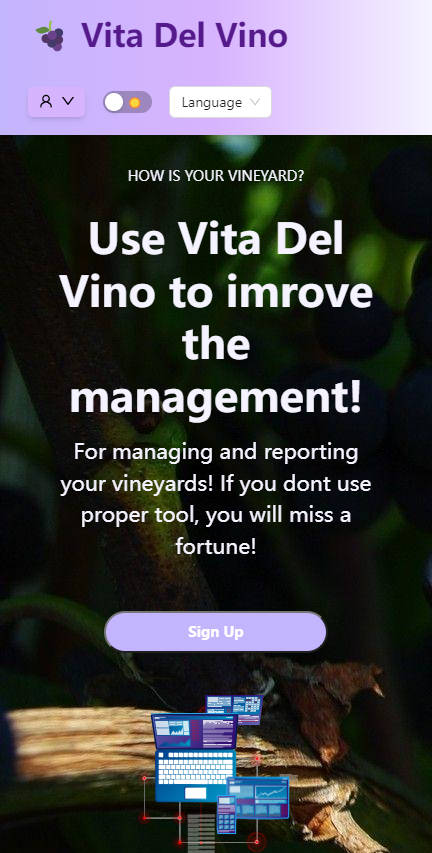
\includegraphics[width=0.5\linewidth]{images/responsive.jpg}
                    \caption{Landing Page on Mobile device}
                    \label{fig:responsive}
                \end{figure}

          \end{enumerate}
\end{enumerate}
\subsection{5.3 Databases}

The database structure for the project is defined using POSTgres GIS and consists of the following tables:

\begin{itemize}
    \item \textbf{areas}: Contains information about different areas, including ID, name, creation timestamp, code, and geometry.
    \item \textbf{companies}: Stores company details such as ID, company name, password, email, phone, creation timestamp, update timestamp, and role ID.
    \item \textbf{areas\_companies\_companies}: Represents the relationship between areas and companies.
    \item \textbf{roles}: Defines different roles with ID and name.
    \item \textbf{interventions}: Holds data about interventions, including ID, type, and description.
    \item \textbf{vineyards}: Contains details about vineyards, including ID, name, winetype, area ID, creation timestamp, geometry, company ID, year of planning, execution details, and area number.
    \item \textbf{interventions\_vineyards\_vineyards}: Represents the relationship between interventions and vineyards.
    \item \textbf{reports}: Stores report information such as ID, title, description, disease, area ID, company ID, vineyard ID, creation timestamp, update timestamp, deletion timestamp, and status.
\end{itemize}

\subsubsection{Structure of Databases}

The conceptual schema is represented by the SQL code, which defines the tables, their columns, and the relationships between them. The logical schema translates this conceptual schema into the actual database tables, columns, and relationships.

\begin{figure}[htbp]
    \centering
    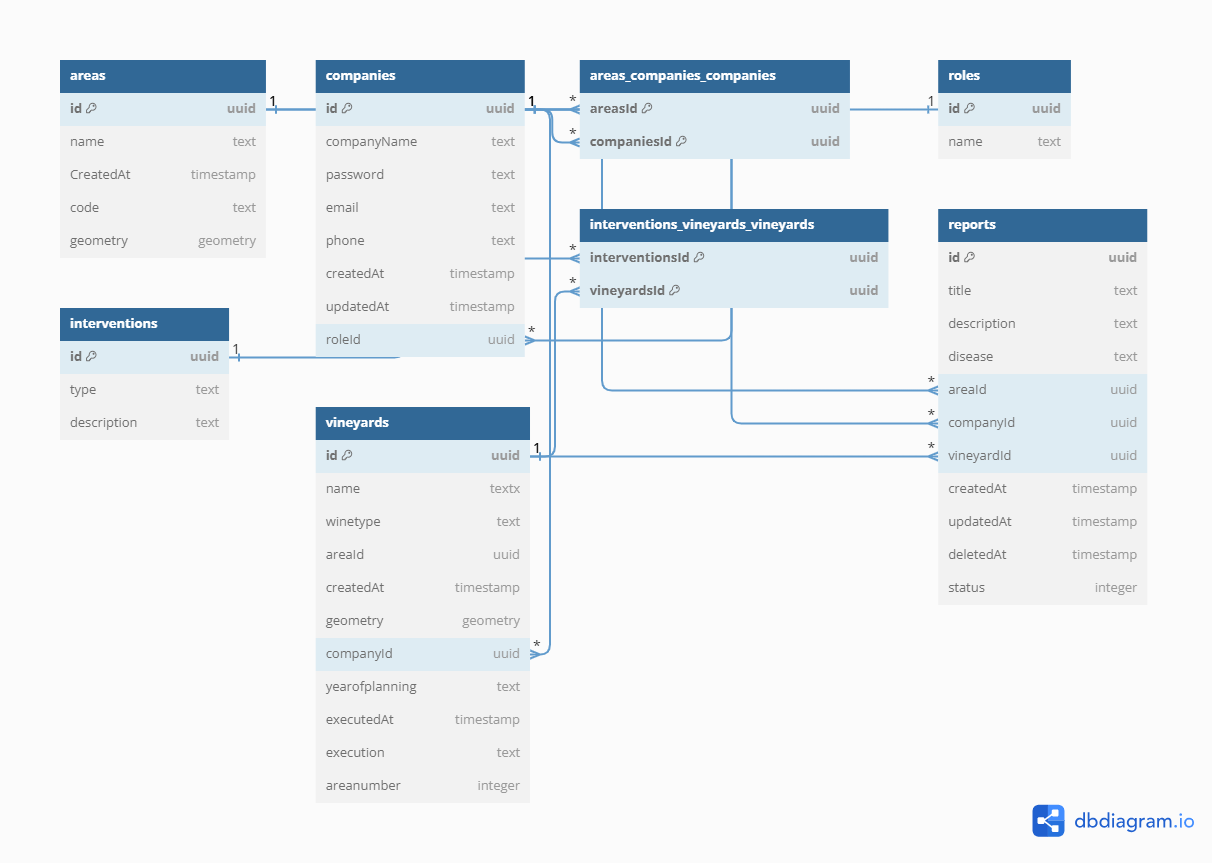
\includegraphics[width=\textwidth]{images/database.png}
    \caption{Database Relational Schema}
    \label{fig:database_schema}
\end{figure}

\subsubsection{Data Volumes}

The data volumes in each table may vary based on the actual usage and input data. Monitoring and optimizing data volumes will be part of the ongoing maintenance.

\subsubsection{Method of Constitution}

The database is constructed based on the DBML code, defining the tables and their properties. It's then implemented in the chosen database management system.

\subsubsection{Mode of Update}

Data is updated through SQL queries, inserts, updates, and deletions executed within the database management system.



\subsection{5.4 Technological Components}
\subsubsection{5.4.1 Application Software Components: System Functions}
\subsubsection{Front-end Development:}
\begin{itemize}
    \item Implemented responsive UI using React, Tailwind CSS, Ant Design, and Formik.
    \item Integrated OpenStreetView maps to display location information.
    \item Impact: Enhanced user experience and accessibility of the application's front-end.
\end{itemize}

\subsubsection{Back-end Development:}
\begin{itemize}
    \item Utilized NestJS framework to create more than 30 backend APIs for user authentication, areas, vineyards management, and report processing.
    \item Managed backend data storage with TypeORM and PostGIS database.
    \item Impact: Streamlined backend processes, data management, and API interactions.
\end{itemize}
\begin{enumerate}
    \item List of software modules in relation to functions.
    \item Description of each module.
    \item Methods of implementation and maintenance.
    \item Transaction volumes.
\end{enumerate}

\subsubsection{5.4.2 Middleware, Operating System}
\begin{enumerate}
    \item List of needed components.
    \item Identification, description, and justification of the components not present.
    \item Method of acquisition.
    \item Management needs.
\end{enumerate}

\subsubsection{5.4.3 Hardware Components}
\begin{enumerate}
    \item There is no hardware components used in my side. The device for GPS should be provide by customers themselves. If the device needs further implementation with the system such as using API to transfer the data, new changes will be added into this project.
\end{enumerate}

\subsection{5.5 Guidelines}
\begin{enumerate}
    \item Coordination of interventions on:
          \begin{enumerate}
              \item Data. The harmonious management of data is pivotal. This includes ensuring data integrity, security, and accessibility. Coordination efforts involve robust data collection, storage, and retrieval mechanisms, as well as data-sharing protocols to facilitate seamless communication between users and agronomists.
              \item Technology: The choice of technologies plays a vital role in the website's functionality and performance. The technology stack, which includes React, Tailwind CSS, Ant Design, Formik, NestJS, TypeORM, and PostGIS, requires careful coordination to ensure compatibility, scalability, and optimal utilization. Each component must seamlessly integrate into the system to deliver a cohesive user experience.
              \item Organisation.  Coordinating organizational aspects involves defining roles, responsibilities, and workflows. Clear lines of communication and collaboration channels between company users and agronomists are established to ensure efficient issue reporting, resolution, and knowledge sharing. This organizational coordination enhances the website's effectiveness in addressing vineyard-related challenges.
          \end{enumerate}
    \item Critical aspects (technological, organisational, about data).
\end{enumerate}
\begin{enumerate}

    \item Technological Aspects: The project's success is deeply intertwined with its technological components. The selection and implementation of React for the frontend, Tailwind CSS and Ant Design for user interface design, Formik for form management, NestJS for the backend, TypeORM for database integration, and PostGIS for geospatial data are critical technological decisions. These aspects must be continuously monitored and adapted to stay aligned with evolving technological trends and user needs.

    \item Organizational Aspects: The organizational structure and workflows within the website's ecosystem are equally critical. A well-coordinated team of agronomists and users, clear roles and responsibilities, and efficient communication channels ensure that the platform serves its purpose effectively. Additionally, the project must remain agile and responsive to changing organizational dynamics and user requirements.

    \item Data Aspects: Data is the lifeblood of the website. Ensuring data accuracy, security, and compliance with regulations is paramount. Coordinated data management practices include data collection, storage, retrieval, and analysis. Moreover, robust data governance policies are essential to maintain data quality and privacy, fostering trust among users and agronomists.

\end{enumerate}
\subsection{5.6 Deployment Plan}

The deployment plan for the project involves the following key aspects:

\begin{enumerate}
    \item \textbf{Definition of Main Phases:} The deployment will encompass several phases, including frontend development, backend development, testing, user training, and final launch.

    \item \textbf{Definition of Resources by Phase:} The resources allocated for each phase will be determined based on project requirements. Frontend development will involve UI/UX designers and React developers, while backend development will require NestJS developers and database administrators.

    \item \textbf{Overall Schedule:} The project is scheduled to be completed within 12 months, starting from the design phase and concluding with the final launch and monitoring phase.

    \item \textbf{Monitoring Mechanisms:} Throughout the deployment, regular monitoring and feedback mechanisms will be established. This includes continuous communication with the development teams, regular testing and quality assurance, and user feedback collection.
\end{enumerate}



\subsection{5.7 Organisational Aspects}

The organisational aspects of the project include the following considerations:

\begin{enumerate}
    \item \textbf{Processes Re-engineering Needs/Opportunities:} The introduction of the new vineyard survey system offers an opportunity to re-engineer existing processes related to disease management, intervention planning, and collaboration between agronomists and vineyard managers. This involves mapping out existing processes, identifying bottlenecks, and designing more streamlined workflows.

    \item \textbf{Organisational Changes:} The project's implementation may lead to changes in the roles and responsibilities of agronomists, vineyard managers, and other stakeholders. Clear communication and training will be necessary to ensure a smooth transition and adoption of the new system.

    \item \textbf{Training Needs:} Training sessions will be organized for agronomists, vineyard managers, and other users to familiarize them with the new system's features and functionalities. Training will cover data input, disease tracking, intervention planning, and reporting.

    \item \textbf{Needs for Support to the System (IT Technical Resources):} The system's ongoing operation will require IT technical resources for maintenance, troubleshooting, and updates. This includes ensuring data security, addressing technical issues, and providing user support.
\end{enumerate}

\subsection{5.8 Risk Management}

The project's risk management strategy involves:

\begin{enumerate}
    \item \textbf{Project’s Risk Profile:} Identified risks include potential data privacy breaches, user resistance to change, technical challenges during development, and unforeseen issues during deployment.

    \item \textbf{Actions on Factors to Reduce Risk:} To mitigate data privacy risks, stringent security measures will be implemented. User resistance will be addressed through comprehensive user training and stakeholder engagement. Technical challenges will be tackled through close collaboration with technology experts.

    \item \textbf{Guidelines for the Management of the Project:} The project will be managed using an agile methodology, allowing for continuous feedback, iterative development, and risk assessment at each stage.

    \item \textbf{Needs for Support to the System (IT Technical Resources):} IT technical resources will be required post-launch to address any technical issues, ensure data integrity, and provide user support.
\end{enumerate}

\subsection{5.9 Benefits Evaluation}

The benefits evaluation will be conducted post-launch to assess the project's impact on disease management, efficiency, collaboration, and vineyard health. Key performance indicators (KPIs) will include disease detection rates, intervention effectiveness, user satisfaction, and reduction in disease-related losses.

\subsection{5.10 Cost Evaluation}

The cost evaluation will encompass development costs, deployment costs, user training costs, and ongoing maintenance costs. This comprehensive assessment will ensure that the project's financial investment aligns with the expected benefits.

\subsection{5.11 Cost/Benefit Analysis}

The cost/benefit analysis will compare the projected benefits of the system (such as improved disease management, increased efficiency, and enhanced collaboration) against the estimated costs (including development, deployment, training, and maintenance). This analysis will provide a holistic view of the project's value proposition.






